\label{sec:simplemodel}
This section investigates the effect of a network externality on the
evolutionary stag hunt game. The following situation is inspired by an
example given in \textcite{kandori_learning_1993}. 
Consider students in university being assigned to
projects in their classes with other students at university. 
Nowadays, most of the projects involve some kind of software tool to either 
present the results, analyze the subject or just manage the process of aggretating 
knowledge. Usually the choice of the tools can be simplified to 
the choice of proprietary software or open source software. 
Both software types are capable of producing the same output for the
projects, but propiertary software has high license costs.
Common examples of this are Open Office vs. Microsoft Word for text editing,
Python vs. Matlab for scientific computing and R vs. Stata for statistical
analysis. Assigned to a project, students can either choose proprietary
software denoted as strategy 1 or open software denoted as strategy 2.
If both students choose open source software they receive utility $a$.
Coordinating on propierty software leaves both with a utility $d$ which is
smaller than $a$ as they have to pay for the licenses. In the case 
where students fail to coordinate on a software tool, the student
with proprietary software gets $c$. However, the other student
has to transfer his contributions to the standards of the proprietary software
as portability is usually only possible in this direction and hence, only 
gets $b$. The parameters fullfill the condition $a < c \geq d <b$.
The structure of the game is precisely that of a stag hunt game. 
Coordination on open source software is the payoff-dominant Nash equilibrium,
but it is risk-dominated by the equilibrium where the students coordinate on
proprietary software. 

For simplification, assume that during their studies, a large body of 
homogenous students is randomly paired by their professor into groups of two 
for a project, implicitly playing the coordination game outlined. 
Concerning the behavior of an individual student, I assume that they are 
not perfectly rational and do not adjust their software choice 
each time they have to do a project.
For simplicity, students in this model behave according to the 
revision protocol of pairwise proportional imitation discussed in section 
\ref{sec:revisionprotocols}. 
This applies, as students tend to use software they always used and 
only change it, if they get to know someone being more successful with
another software choice. Therefore, the dynamic in the model can be 
described by the replicator dynamic derived for the stag hunt game in 
equation \eqref{eq:replicatorpara}.
This model would not differ in terms of convergence and stability of Nash 
equilibria to the evolutionary stag hunt game above.

However, I want to introduce \textit{network externalities} in this model. 
The interest of the economic literature turned to open source software 
development, because it is commonly observed that users contribute to 
projects without receiving a monetary payment for it.
In fact users share their source code publicly to the open source community,
being motivated by peer recognition and the signaling for career concerns
\parencite[21]{lerner_simple_2002}.
The utility for a user increases with the size of the community as 
more people contributing code enhance the variety and usefulness of the 
software. 
To incorporate this in the model, let the utility for a student 
in the case of coordination on open source software be a function of 
population size using that strategy $f(x)$. 
Preserving the general structure of the
game, it is useful to focus on the functional specification 
$f(x) = a + e(x)$, where $a$ is the payoff parameter used 
previously and $e(x)$ denotes the network externality. 
A positive network externality satisfies $e(x)\geq 0$ and 
$\frac{de(x)}{dx}>0$, 
as an increase of the population share choosing the strategy
also increases the utility due to the network. 
Including the parameter $a$ ensures that the utility of this 
strategy combination is never below the utility of coordination on 
proprietary software. Otherwise, the structure of the stage game would 
differ fundamentally with respect to the population share choosing strategy 
one. The payoff matrix, using local shifts, is 
$A=\begin{psmallmatrix}\alpha_1+u(x) && 0 \\ 0&& \alpha_2\end{psmallmatrix}$. 
Substituting into the replicator dynamic  \ref{eq:replicatorpara} yields:
\begin{alignat}{2}
        \dot{x} = \varphi(x) = x^2(\alpha_1+e(x) +2\alpha_2 ) 
        - x^3(\alpha_1+e(x)+\alpha_2) - x(\alpha_2)
        \label{eq:externalitymodel}
\end{alignat}
By plugging $x=0$ and $x=1$ into equation \eqref{eq:externalitymodel} and, 
by applying the linearization theorem, one can ensure 
that the fixed point with pure strategies and their
property of asymptotical stability did not change
($\varphi'(1) = -\alpha_1 -e(1),\ \varphi'(0) = -\alpha_2 -e(0)$).
The literature on network externalities usually assumes a diminishing
marginal effect of the network externality $\frac{d^2e(x)}{dx^2} <0$ 
\parencite[73]{lin_impact_2008}. However, the analysis presented in this text
will focus on the linear form $e(x) = \beta x$ with the externality parameter
$\beta \in \realnumb_+$. This restriction does not change the main implication
of the model. 
Despite not changing the stability of the pure states, 
the externality affected the inner fixed point of the dynamic.
The polynominal $\varphi(x)$ is now of degree $4$:
\begin{align}
        \dot{x} = \varphi(x) = -\beta x^4 -x^3(\alpha_1 + \alpha_2 
        - \beta ) + x^2 (\alpha_1 + 2 \alpha_2) - x(\alpha_2)
\end{align}
Using the knowledge from the general case, we can find the roots, i.e. fixed
points of the dynamic, by reducing the degree with the two roots known. The
polynominal of degree $2$ can then be solved applying a quadratic formula\footnote{
The solution with negative sign was omitted, since it has no economic 
interpretation.}, so that the fixed point with a mixed population state is
$x_3 = -\frac{\alpha_1+\alpha_2}{2 \beta} + 
\sqrt{\frac{(\alpha_1+\alpha_2)^2}{4\beta^2} +\frac{\alpha_2}{\beta}}$. 
The new inner fixed point is always lower than the inner fixed point without 
externality, but does never coincide with the stag hunt equilibrium, as it 
satisfies $0<x_3<\frac{\alpha_2}{\alpha_1+\alpha_2}$. 
Taking the limit $\lim_{\beta \rightarrow 0} x_3 = 
\frac{\alpha_2}{\alpha_2+\alpha_1}$ verifies the intuition that for a 
diminishing network externality parameter the model without 
externality is obtained.
The plot of the dynamic and the polynominal is 
shown in figure \ref{fig:plotmodellinear}.
Note that the share of students choosing strategy 1 is now lower at the 
inner fixed point, displayed by the gray dashed lines in subfigure 
\ref{fig:externalitypolynominal}, showing that the externality has a positive 
effect on the attractiveness of choosing open source software. 
Indeed, the basin of attraction of the equilibrium in which all 
students are using open source software became larger, 
depicted by the distance to the inner fixed point.
This is illustated by the dashed, red horizontal line, 
the inner fixed point without externality, and the dashed, green horizontal 
line, the inner fixed point with externality, 
in figure \ref{fig:dynamiclinear}.
\begin{figure}[h]
        \centering
        \begin{subfigure}{.5\textwidth}
        \centering
        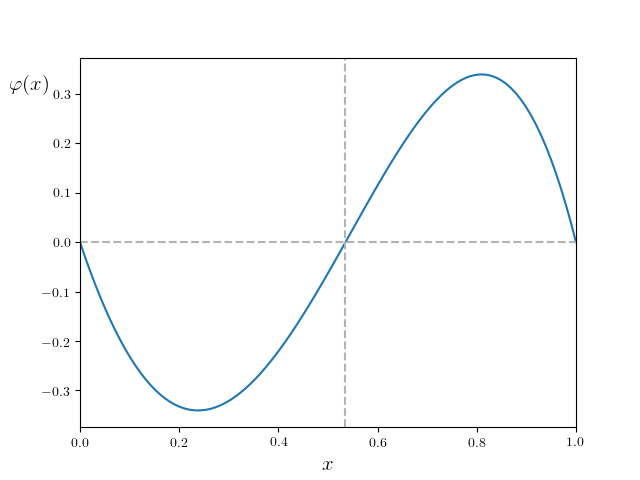
\includegraphics[scale=0.5]{polynominallinearmodel.pdf}
        \caption[Polynominal of the externality model]{The polynominal $\varphi(x)$} 
        \label{fig:externalitypolynominal}
        \end{subfigure}%    
        \begin{subfigure}{.5\textwidth}
        \centering
        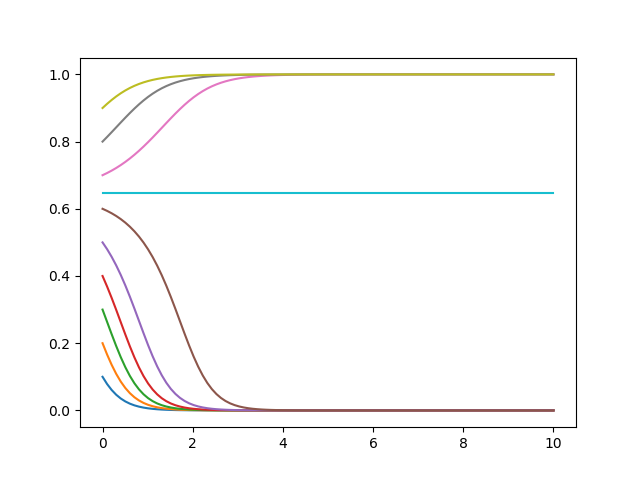
\includegraphics[scale=0.5]{dynamiclinearmodel.pdf}
        \caption[Replicator dynamic of the model with externality]{The dynamic $x(t)$ for different $x(t=0)$} 
        \label{fig:dynamiclinear}
        \end{subfigure}%        
        \caption[Polynominal and Dynamic of the model with externality]
        {The linear externality 
                model for parameters $\alpha_1=1,\alpha_2=3,\beta=3$}
        \label{fig:plotmodellinear}
\end{figure}
The basins of attraction have equal size for $\beta^* = 2 (\alpha_2 -\alpha_1)$,
attracting an equal amount of initial conditions. However,
the proprietary equilibrium looses its risk-dominance property 
only for $1 > x > \frac{\alpha_2-\alpha_1}{\beta}  $, using definition 
\ref{eq:riskdom}. The right hand side of the equation must be lower than one 
to change the risk-dominance property. This leads to the conclusion 
that in this model, the size of the basin of attraction and the risk-dominance
property do not coincide in general, since the externality changes the Nash 
product associated with the pure strategy 1 equilibrium. Consider for example 
the parameter setting $\alpha_1 =1, \alpha_2=3$, but now let $\beta=3$. 
The basin of attraction is not equal, since $3<\beta^*= 4$. 
The open source equilibrium attracts all trajectories starting with 
$x_0 \in (\frac{-2+\sqrt{13}}{3},1]$ and hence the proprietary equilibrium attracts
all trajectories with $x_0 \in [0,\frac{-2+\sqrt{13}}{3})$. 
Clearly, the latter basin of 
attraction is larger ($\frac{-2+\sqrt{13}}{3}>0.5)$, 
but the open source equilibrium gets risk-dominant for
$x>\frac 23$. This implies that the network externality not only increases the
utility obtained from the choice of open source software, but also,
combined with a high enough user base, makes this choice risk-dominant. 

The model presented here is a simplification of the real world. 
First, the students are expected to be able to review which software is 
appropriate for their projects, hence have more information available than 
assumed in the model. Secondly, talking to their fellow student seems
possible before deciding which software to use for the project. 
However, as the experimental literature that will be discussed in section 
\ref{sec:experimentalevidence}, and \textcite{aumann_nash_1990} suggest, 
cheap talk does not generally solve the coordination problem. 
Additionally, the way the attractiveness of a strategy increases with
the population size, the network externality, is modeled quite naively.
Students at university and social networks in general are not fully
connected as students, for example, only do projects with fellow students
in the same classes. Furthermore, students usually try to do projects
with people they are socially connected with. In fact, the assumption about
a fully connected network is ``one of the main criticisms of evolutionary game
theory'' \parencite{hanauske_evolutionare_2011}. 
As a consequence, many researchers recently gave attention to the 
structure of the network underlying the interaction of agents and 
evolving of network structure \parencite[46]{szabo_evolutionary_2007}.
For example, \textcite{ohtsuki_simple_2006} found 
that fewer connectivity 
leads to more cooperation for a range of network topologies,
agreeing with the intuition
``The fewer friends I have the more strongly my fate is bound to theirs'' 
\parencite[1]{ohtsuki_simple_2006}.
Although the model with a positive linear network externality is far too 
simple to capture the effect of complex, adapting networks, it gives an 
intuition of how coordination of a small group, in this case two players, 
can be affected by the choice of the whole population, as it changes
the structure of the coordination game they play.
